\PassOptionsToPackage{dvipsnames}{xcolor}
\documentclass[mathserif]{beamer}

\usepackage{tgadventor}
\usepackage[absolute,overlay]{textpos}

\usepackage{listings}
\definecolor{light-gray}{gray}{0.9}
\lstset{columns=fullflexible, 
        basicstyle=\ttfamily\footnotesize,
        breaklines=true,
        backgroundcolor=\color{light-gray},
        xleftmargin=0.5cm,
        frame=tlbr,
        framesep=4pt,
        framerule=0pt}


% approx symbol
\usepackage{textcomp}
\newcommand{\textapprox}{\raisebox{0.5ex}{\texttildelow}}


\title{Correlated Models of Discrete Charcter Evolution in \texttt{RevBayes}}
\author{Will Freyman}
\institute{
  Department of Ecology, Evolution \& Behavior \\
  University of Minnesota \\
  \medskip
  \color{Emerald}willfreyman@gmail.com \\
  http://willfreyman.org

}
\date{UC Berkeley Workshop, February 26-27 2018}


\beamertemplatenavigationsymbolsempty

\setbeamercolor{alerted text}{fg=Emerald}


\begin{document}


\frame{\titlepage}


\begin{frame}[fragile]
    \begin{block}{Correlated evolution of discrete characters:}
    \bigskip
    \begin{center}
    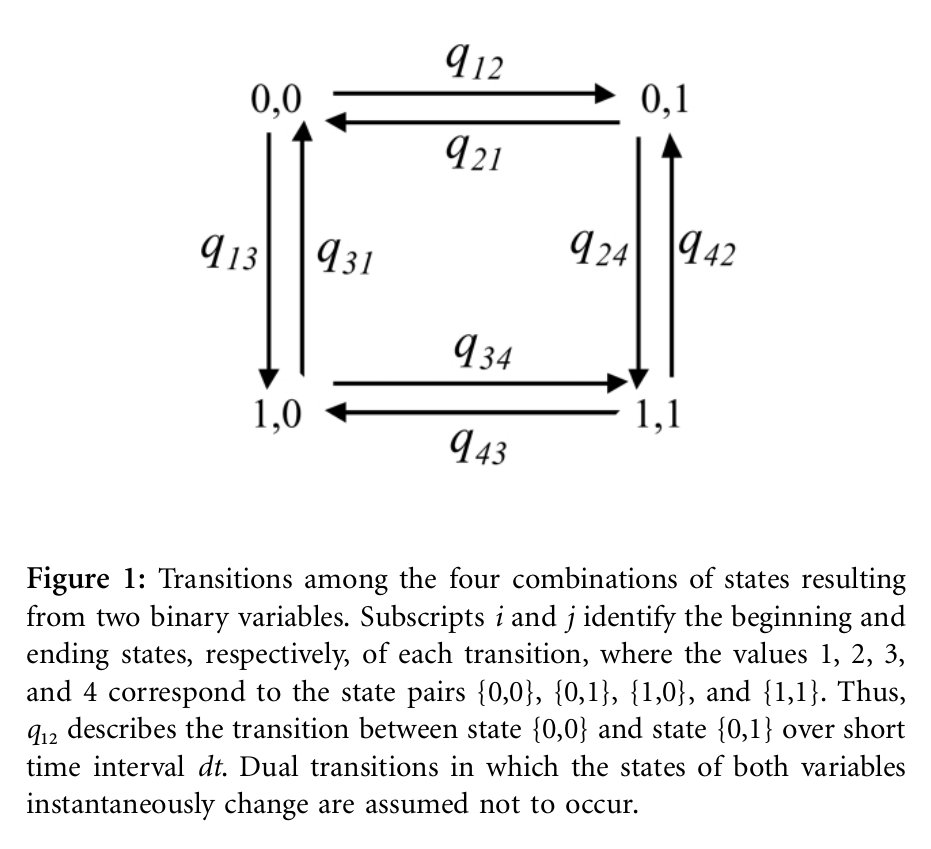
\includegraphics[scale=0.2]{figures/pagel1.png}\\
        \medskip
    \end{center}
    \end{block}
    \begin{textblock*}{10cm}(1cm,9cm)
    \tiny Image from Pagel and Meade (2006)
    \end{textblock*}
\end{frame}


\begin{frame}[fragile]
    \begin{block}{Correlated evolution of discrete characters:}
    \bigskip
    \begin{center}
    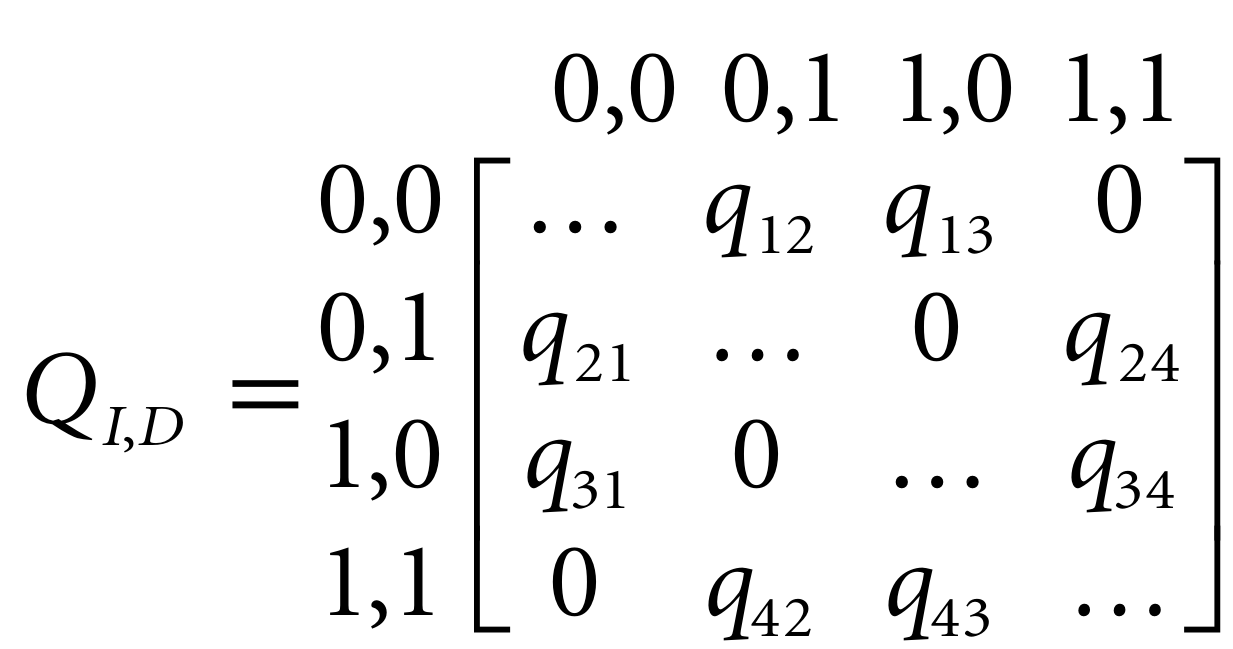
\includegraphics[scale=0.15]{figures/pagel2.png}\\
        \bigskip
        \bigskip
        For a fully independent model:
        $q_{12} = q_{34}$, 
        $q_{13} = q_{24}$, 
        $q_{21} = q_{43}$, and 
        $q_{31} = q_{42}$. 
    \end{center}
    \end{block}
    \begin{textblock*}{10cm}(1cm,9cm)
    \tiny Image from Pagel and Meade (2006)
    \end{textblock*}
\end{frame}


\begin{frame}[fragile]
    \begin{block}{Correlated evolution of discrete characters:}
    \bigskip
        We can test the fit of the independent model to a dependent model
        using either \alert{Bayes factors} or \alert{reversible-jump MCMC}.\\
    \bigskip
        \begin{itemize}
           \item \texttt{src/independent\_Bayes\_factors.Rev}
           \item \texttt{src/correlated\_Bayes\_factors.Rev}
           \item \texttt{src/correlated\_reversible\_jump.Rev}
        \end{itemize}
    \end{block}
    \begin{textblock*}{10cm}(1cm,9cm)
    \tiny Image from Pagel and Meade (2006)
    \end{textblock*}
\end{frame}


\begin{frame}[fragile]
    \begin{block}{Correlated evolution of discrete characters:}
    \bigskip
        Here we will calculate the marginal likelihood for the most general model of correlated trait evolution 
        described in Pagel and Meade (2006). They notated it as \texttt{(1,2,3,4,5,6,7,8)}.\\
    \bigskip
    Read in the tree and tip data:\\
    \bigskip
    \begin{lstlisting}
tree_obs <- readTrees("data/phylo.tree")[1]
morph_data <- readCharacterData("data/correlated.nex")
    \end{lstlisting}
    \end{block}
\end{frame}


\begin{frame}[fragile]
    \begin{block}{Correlated evolution of discrete characters:}
    \bigskip
The character state transition rate matrix\\
    \bigskip
    \begin{lstlisting}
q_12 ~ dnExponential(10)
q_13 ~ dnExponential(10)
q_21 ~ dnExponential(10)
q_24 ~ dnExponential(10)
q_31 ~ dnExponential(10)
q_34 ~ dnExponential(10)
q_42 ~ dnExponential(10)
q_43 ~ dnExponential(10)
Q_morph := fnFreeK([q_12, q_13, 0, q_21, 0, q_24, q_31, 0, q_34, 0, q_42, q_43], rescaled=FALSE)
    \end{lstlisting}
    \end{block}
\end{frame}


\begin{frame}[fragile]
    \begin{block}{Correlated evolution of discrete characters:}
    \bigskip
 root frequencies:
    \bigskip
    \begin{lstlisting}
pi_morph ~ dnDirichlet([1,1,1,1])
    \end{lstlisting}
    \bigskip
The phylogenetic CTMC:
    \bigskip
    \begin{lstlisting}
ctmc_morph ~ dnPhyloCTMC(tree_obs, Q=Q_morph, rootFrequencies=pi_morph, nSites=1, type="Standard")
ctmc_morph.clamp(morph_data)
    \end{lstlisting}
    \end{block}
\end{frame}

\begin{frame}[fragile]
    \begin{block}{Correlated evolution of discrete characters:}
    \bigskip
Just like before, we need to specify the model, moves, monitors.\\
    \bigskip
    \begin{lstlisting}
mymodel = model(ctmc_morph)

moves[1] = mvScale(q_12)
moves[2] = mvScale(q_13)
moves[3] = mvScale(q_21)
moves[4] = mvScale(q_24)
moves[5] = mvScale(q_31)
moves[6] = mvScale(q_34)
moves[7] = mvScale(q_42)
moves[8] = mvScale(q_43)
moves[9] = mvSimplexElementScale(pi_morph)

monitors[1] = mnScreen(printgen=10)
    \end{lstlisting}
    \end{block}
\end{frame}


\begin{frame}[fragile]
    \begin{block}{Correlated evolution of discrete characters:}
    \bigskip
Yesterday we ran MCMC analyses. For Bayes factor calculations
we need to compute the marginal likelihood of the model so
we run a power posterior analysis:\\
    \bigskip
    \begin{lstlisting}
pow_p = powerPosterior(mymodel, moves, monitors, "output/correlated.out", cats=50)
pow_p.burnin(generations=100, tuningInterval=10)
pow_p.run(generations=100)
    \end{lstlisting}
    \bigskip
The calculate the marginal likelhood:\\
    \bigskip
    \begin{lstlisting}
ss = steppingStoneSampler(file="output/correlated.out", 
                          powerColumnName="power", 
                          likelihoodColumnName="likelihood")
ss.marginal()
    \end{lstlisting}
    \end{block}
\end{frame}


\begin{frame}[fragile]
    \begin{block}{Correlated evolution of discrete characters:}
    \bigskip
We can similarly set up the most general \alert{independent}
        model described in Pagel and Meade (2006) which they notated \texttt{((1,1,2,2,3,3,4,4)}.
 It is exactly the same, except for the rate matrix:\\
    \bigskip
    \begin{lstlisting}
q_12 ~ dnExponential(10)
q_13 ~ dnExponential(10)
q_21 ~ dnExponential(10)
q_24 := q_13
q_31 ~ dnExponential(10)
q_34 := q_12
q_42 := q_31
q_43 := q_21
Q_morph := fnFreeK([q_12, q_13, 0, q_21, 0, q_24, q_31, 0, q_34, 0, q_42, q_43], rescaled=FALSE)
    \end{lstlisting}
\bigskip
Don't forget to remove the moves for the rates that are now deterministic.\\
    \end{block}
\end{frame}




\begin{frame}[fragile]
    \begin{block}{Correlated evolution of discrete characters:}
    \bigskip
The marginal likelihoods I got were -19.3 for the independent model
and -17.9 for the correlated model.\\
    \bigskip
        Since -17.9 + 19.3 = 1.4, this means the 2\textit{ln}BF = 3.8, which is positive support for
        the correlated model over the independent model (Kass and Raftery 1995).\\
    \bigskip
        However, we only examined one of the many possible different correlated models
        of character evolution.
        It is possible that some of the character state transitions
        are dependent on one another and others are not. We can test for these using
        reversible-jump MCMC.\\
    \end{block}
\end{frame}

\begin{frame}[fragile]
    \begin{block}{Correlated evolution of discrete characters:}
    \bigskip
    \bigskip
    \bigskip
We can use reversible-jump MCMC over rate multipliers which will allows
        every pair of rates described in the indepedent model
        to no longer be set equal.\\
    \bigskip
This is a simple modification to the independent model we previously specified
        for the Bayes factor calculation.
    \end{block}
\end{frame}


\begin{frame}[fragile]
    \begin{block}{Correlated evolution of discrete characters:}
    \bigskip
        Each multiplier will have the
value 1.0 or a value drawn from a log uniform distribution
varying from 0.02 to 55.\\
    \bigskip
    \begin{lstlisting}
m_13 ~ dnReversibleJumpMixture(constantValue=0,
                               baseDistribution=dnUniform(-4, 4),
                               p=0.5)
m_12 ~ dnReversibleJumpMixture(constantValue=0,
                               baseDistribution=dnUniform(-4, 4),
                               p=0.5)
m_31 ~ dnReversibleJumpMixture(constantValue=0,
                               baseDistribution=dnUniform(-4, 4),
                               p=0.5)
m_21 ~ dnReversibleJumpMixture(constantValue=0,
                               baseDistribution=dnUniform(-4, 4),
                               p=0.5)
    \end{lstlisting}
\bigskip
    \end{block}
\end{frame}


\begin{frame}[fragile]
    \begin{block}{Correlated evolution of discrete characters:}
    \bigskip
We use deterministic nodes to monitor posterior probabilities of each 
transition being dependent (correlated) as opposed to independent:
    \bigskip
    \begin{lstlisting}
cor_13_24 := ifelse(m_13 != 0, 1, 0)
cor_12_34 := ifelse(m_12 != 0, 1, 0)
cor_31_42 := ifelse(m_31 != 0, 1, 0)
cor_21_43 := ifelse(m_21 != 0, 1, 0)
    \end{lstlisting}
\bigskip
    \end{block}
\end{frame}


\begin{frame}[fragile]
    \begin{block}{Correlated evolution of discrete characters:}
    \bigskip
When we set up a rate matrix we must include the rate multipliers:
    \bigskip
    \begin{lstlisting}
q_12 ~ dnExponential(10)
q_13 ~ dnExponential(10)
q_21 ~ dnExponential(10)
q_24 := q_13 * exp(m_13)
q_31 ~ dnExponential(10)
q_34 := q_12 * exp(m_12)
q_42 := q_31 * exp(m_31)
q_43 := q_21 * exp(m_21)
Q_morph := fnFreeK([q_12, q_13, 0, q_21, 0, q_24, q_31, 0, q_34, 0, q_42, q_43], rescaled=FALSE)
    \end{lstlisting}
\bigskip
    \end{block}
\end{frame}


\begin{frame}[fragile]
    \begin{block}{Correlated evolution of discrete characters:}
    \bigskip
And we must also add MCMC moves for the rate multipliers:
    \bigskip
    \begin{lstlisting}
moves[6] = mvSlide(m_13)
moves[7] = mvSlide(m_12)
moves[8] = mvSlide(m_31)
moves[9] = mvSlide(m_21)
moves[10] = mvRJSwitch(m_13)
moves[11] = mvRJSwitch(m_12)
moves[12] = mvRJSwitch(m_31)
moves[13] = mvRJSwitch(m_21)
    \end{lstlisting}
\bigskip
    \end{block}
\end{frame}


\begin{frame}[fragile]
    \begin{block}{Correlated evolution of discrete characters:}
    \bigskip
    \bigskip
After running the MCMC analysis view the results in Tracer.\\
    \bigskip
We see that the posterior probability of 
transitions being independent are low.\\
    \bigskip
Once one character goes from $0\rightarrow1$
        the other character also goes from $0\rightarrow1$
with a very high rate.
\bigskip
    \end{block}
\end{frame}

\end{document}
